\documentclass[a4paper,11pt]{article}
\usepackage[left=2.5cm, right=2.5cm, top=2cm, bottom=2.5cm]{geometry}
\usepackage{graphicx}
\usepackage{amssymb}
\usepackage{amsmath}
\usepackage{wrapfig}

\begin{document}
\title{\LARGE{\textbf{ECEN 203 Lab 4}\\SPICE 2}}
\author{Niels Clayton : 300437590}
\date{}
\maketitle

\section*{3 - Resonant Frequency}
The transfer function of the provided circuit is:\\
$\dfrac{R_{1}}{R_{1}+j(\dfrac{-1}{\omega C}+ \omega L)}$\\
In order to produce the greatest response from this circuit, the term $\dfrac{-1}{\omega C}+ \omega L$ must be equal to zero. When this term is zero, $\omega$ will be at the resonant frequency.\\
$\omega = \dfrac{1}{\sqrt{LC}}$\\
$\omega = \dfrac{1}{\sqrt{47n \times 220m}} = 1984 rads$ or $1565Hz$\\
\begin{figure}[h]
\centering
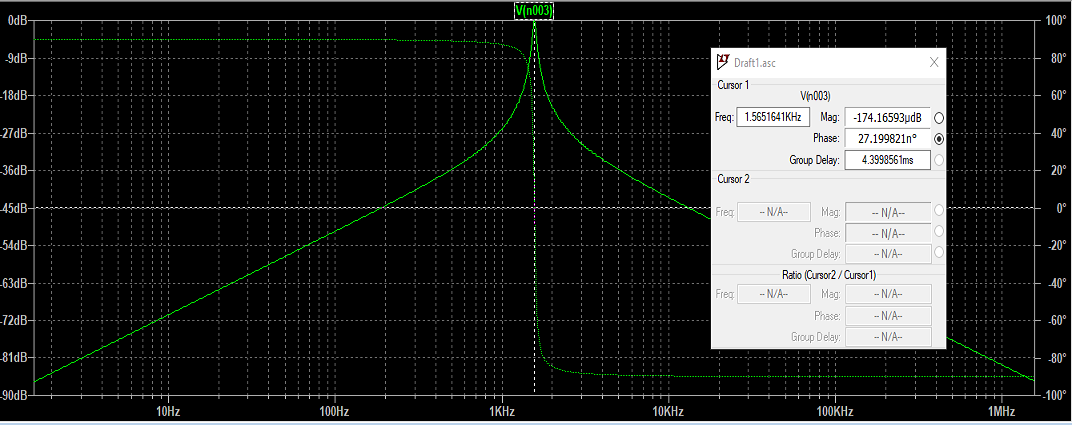
\includegraphics[width=\linewidth]{resonant_frequency.png}
\caption{With a cursor it can be seen the the resonant frequency is $1565Hz$}
\end{figure}
\section*{4 - Q-factor}
$Q_{series} = \dfrac{1}{R}\sqrt{\dfrac{L}{C}} \therefore \dfrac{1}{100}\sqrt{\dfrac{220m}{47n}} = 21.64$\\
Q can also be calcualted using the resonant frequency, and the bandwidth, where bandwidth is the number of passing frequencies (frequencues with less than a 3dB drop).\\
$Q_{series} =\dfrac{f_{res}}{B}$\\
Using cursors we are able to find the passing frequencies:
\begin{itemize}
\item
Frequency 1 = $1.53kHz$
\item
Frequency 2 = $1.60kHz$
\end{itemize}
$Q = 22.63$ Which is very similar to the value calculated before.\\
To produce Q of varying values: 
\begin{itemize}
\item
$Q = 0.25 \rightarrow R = 8654 \Omega$
\item
$Q = 0.5 \rightarrow R = 4327 \Omega$
\item
$Q = \dfrac{1}{\sqrt{2}} \rightarrow R = 3059 \Omega$
\item
$Q = 1 \rightarrow R = 2163 \Omega$
\item
$Q = 10 \rightarrow R = 216 \Omega$
\end{itemize}
Now look at the response of the circuit when varying the resistance with a DC voltage.
\begin{figure}[h]
\centering
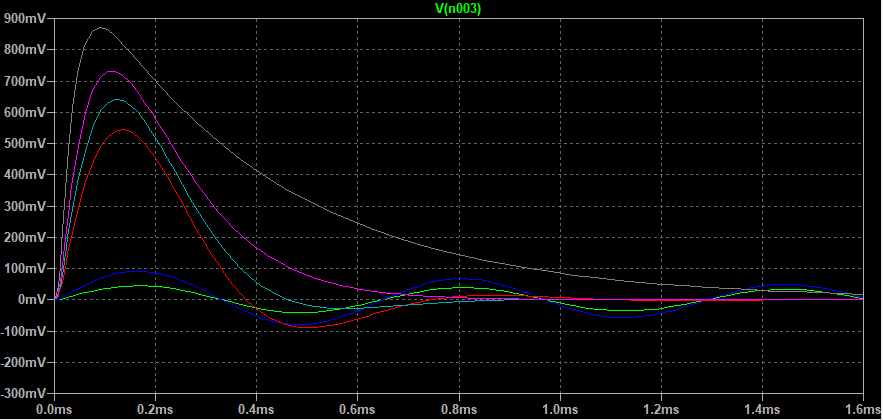
\includegraphics[width=\linewidth]{varing_Resistanc_DC.png}
\end{figure}
As we increase $Q$, We see that the circuit tends to return to a stable state more rapidly with less oscillation. This is the case until the point where $Q < 0.5$ at which point the circuit is over damped, and the size of the resistor is limiting the rate at which the capacitor can discharge. We can also observe that at the point where $Q = 0.5$ the system is "critically" damped, meaning that it returns to a stable state within the shortest time period.
\newpage
\section*{5 - Parameter sensitivity}
\begin{figure}[h]
\centering
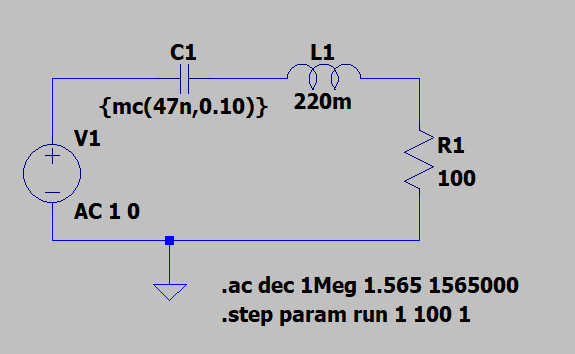
\includegraphics[width=\linewidth]{paramater.png}
\end{figure}
\begin{figure}[h]
\centering
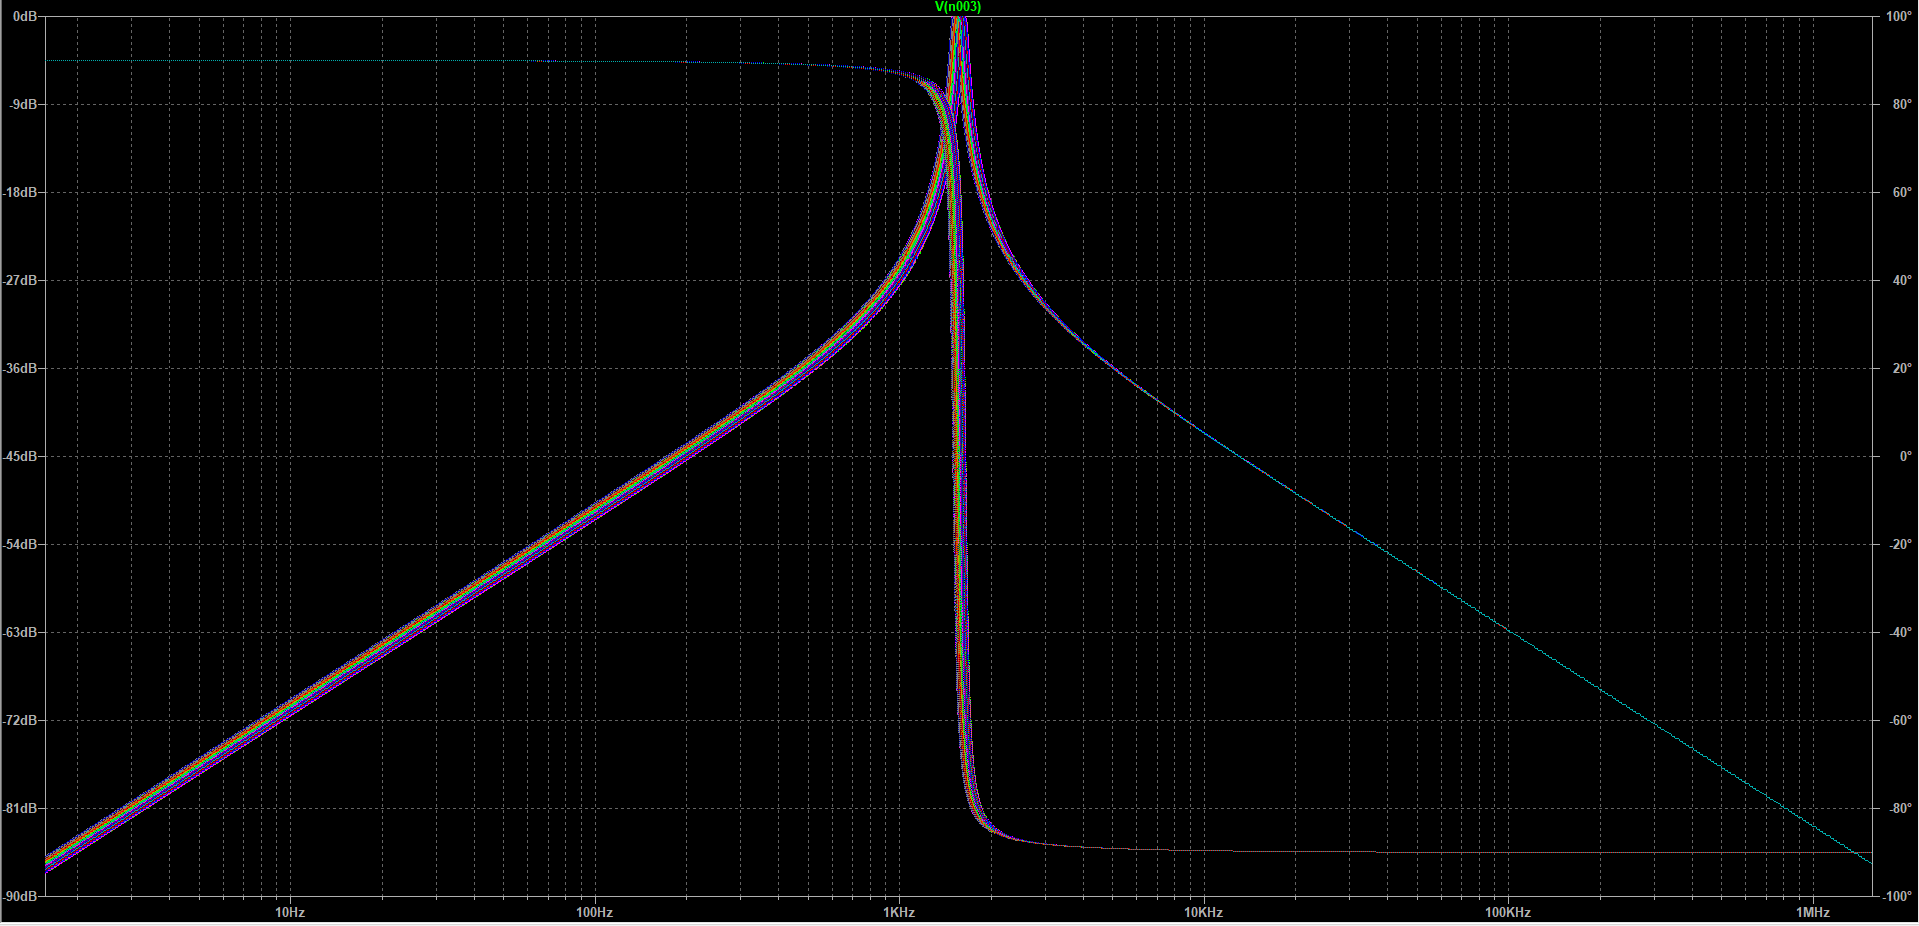
\includegraphics[width=\linewidth]{full.png}
\end{figure}
\begin{figure}[h]
\centering
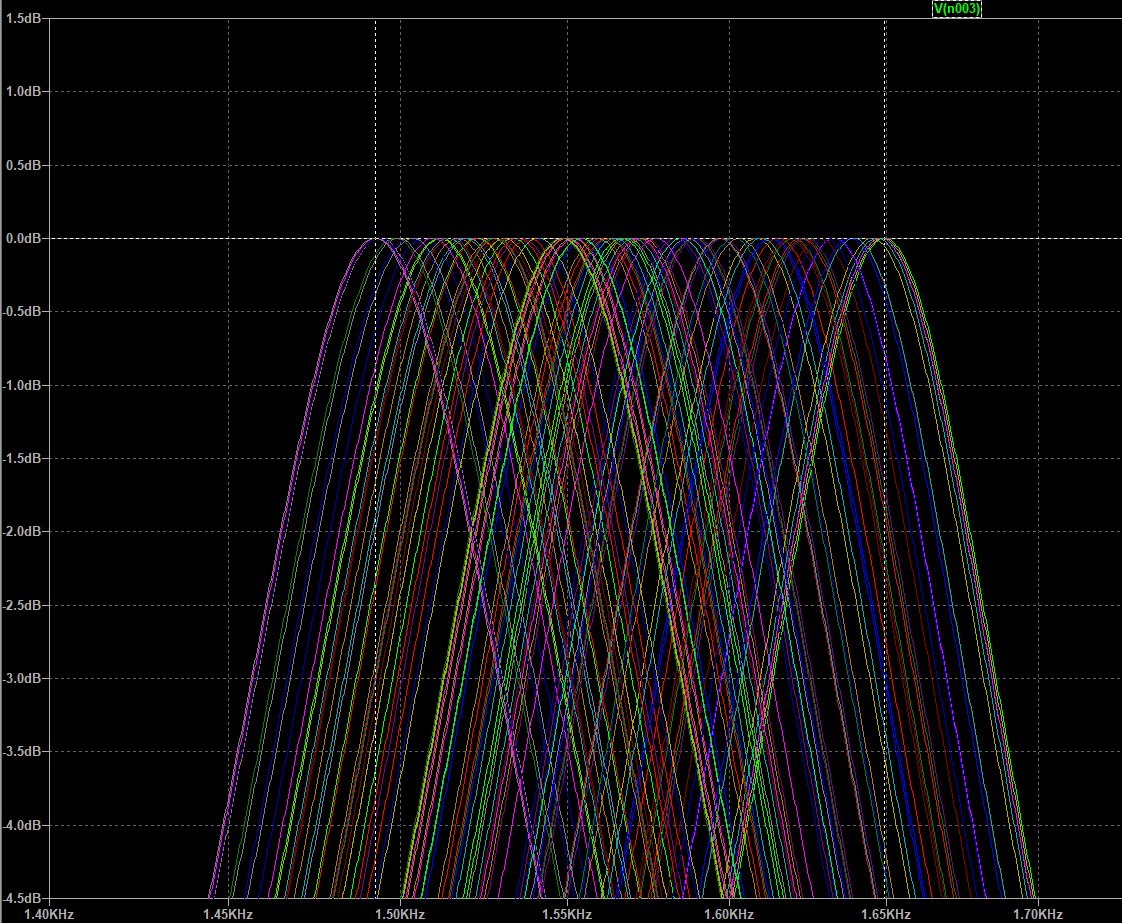
\includegraphics[width=\linewidth]{range.png}
\end{figure}

\end{document}
